% !TEX TS-program = pdflatex
% !TEX root = Tes.tex
% !TEX spellcheck = en-EN

\documentclass[12pt,%                      % corpo del font principale
               a4paper,%                   % A4 papers
               %twoside,openright,%         % twoside with free right side
               oneside,openany,%           % one side
               titlepage,%                 % use a titlepage
               headinclude,footinclude,%  % header and foot header
               BCOR5mm,%                   % rilegatura di 5 mm
               cleardoublepage=empty,%     % empty pages with no header and foot
               tablecaptionabove,%         % table caption above tables
               floatperchapter,
               ]{scrreprt}                 % KOMA-Script report class;


\usepackage{braket}
\usepackage{changepage}
\usepackage[english]{babel}	% latest language is predefined
\usepackage[T1]{fontenc}		% font coding


\usepackage{indentfirst}		% indent first paragraph of each section
\usepackage{mparhack,fixltx2e,relsize}	% fancy typographies stuff

\usepackage[eulerchapternumbers,%	% chapter font Euler
            subfig,%			% in subfig objects
            beramono,%			% Bera Mono as fixed spacing font
            eulermath,%			% AMS Euler as math font
            pdfspacing,%		% improves line filling
            listings,%			% code output
 %          parts,%			% uncomment for a document divided in parts
            listsseparated,
            ]{classicthesis}		% style ClassicThesis
%\setlength{\cftbeforeloftitleskip}{100pt}
%\renewcommand{\cftbeforeloftitleskip}{1000pt}

\usepackage{arsclassica}		% modifies some aspects of ClassicThesis package
\let\marginpar\oldmarginpar		% for margin notes with \todonotes (overwise conflict with the new definition of \marginpar in classic thesis)
\usepackage[shadow]{todonotes}			% for margin notes and comments

\usepackage{bookmark}			% bookmarks

%*********************************************************************************
% Bibliography
%*********************************************************************************
%%\usepackage[style=authoryear,hyperref,backref,natbib, ,maxcitenames=1, mincitenames = 1, citestyle=authoryear-comp, backend=biber,sortcites,sorting=ynt]{biblatex}
%\usepackage[style=numeric,hyperref,backref,natbib]{biblatex}




%*********************************************************************************
% Graphics
%*********************************************************************************
\usepackage{graphicx}			% images
\usepackage{subfigure}
\usepackage{wrapfig}
\usepackage{tikz}
\usetikzlibrary{mindmap,trees}
\usetikzlibrary{backgrounds}
\usepackage{verbatim}
\usepackage[dvipsnames]{xcolor}
% \usepackage{morefloats}
%\usepackage{chngcntr}
\usepackage{pdfpages}

%*********************************************************************************
% Tables
%*********************************************************************************
\usepackage{tabularx}			% table of predefined length
\usepackage{siunitx}
\usepackage{pbox}
\usepackage{colortbl}
\usepackage{multirow}
\usepackage{booktabs}
\usepackage{rotating}
\usepackage{hhline}
\setlength\tabcolsep{3pt}
\usepackage{changepage}
% \usepackage[showframe=true]{geometry}

%*********************************************************************************
% Mathematics and symbols
%*********************************************************************************
\usepackage{amsmath, amssymb, amsthm}	% mathematics stuff
\usepackage{mathrsfs}
\usepackage{calc}
\usepackage{algorithmic}
\usepackage[ruled]{algorithm}
\usepackage{latexsym}
\usepackage[geometry]{ifsym}
\usepackage{mathabx}
\usepackage{pifont}

%*********************************************************************************
% Personal
%*********************************************************************************
\usepackage[font=itshape]{quoting}			% fancy quotation packages. [font=small] old option
\usepackage[english]{varioref}		% complete reference package
\usepackage{hyperref}
\usepackage{url}
\usepackage[intoc, english, noprefix]{nomencl}	%for list of symbols
\usepackage[normalem]{ulem}
\usepackage{chemfig} %for chemical formulas
\usepackage{eurosym}			% euro symbol
\usepackage{epigraph}
\usepackage{calligra}
\usepackage{soul}
\usepackage[utf8]{inputenc}

\definecolor{codegreen}{rgb}{0,0.6,0}
\definecolor{codegray}{rgb}{0.5,0.5,0.5}
\definecolor{codepurple}{rgb}{0.58,0,0.82}
\definecolor{backcolour}{rgb}{0.95,0.95,0.92}


\setlength{\epigraphwidth}{\textwidth}



%*********************************************************************************
% Calling personal settings and making nomenclature
%*********************************************************************************
%*********************************************************************************
% Personal commands
%*********************************************************************************
\newcommand{\myName}{Martina Corsini,Marzio De Corato }	% author
\newcommand{\myTitle}{Association analysis and tweets - Project for the course Algorithms for massive datasets (DSE)}	% title
\newcommand{\myDegree}{Data Science and Economics}	% thesis type
\newcommand{\myUni}{Unimi}	% institute
\newcommand{\myLocation}{Milan}	% place
\newcommand{\myTime}{\today}	% date

%*************************
%Scaling tikz mindmaps
%******************
\makeatletter
\def\hlinewd#1{%
\noalign{\ifnum0=`}\fi\hrule \@height #1 %
\futurelet\reserved@a\@xhline}
\makeatother

%*********************************************************************************
% General math defs
%*********************************************************************************
\newcommand{\beq}{\begin{equation}}
\newcommand{\eeq}{\end{equation}}

\newcommand{\bea}{\begin{eqnarray}}
\newcommand{\eea}{\end{eqnarray}}

\setdoublesep{.5ex}
\renewcommand*\printatom[1]{\ensuremath{\mathsf{#1}}}
\setatomsep{2em}

\newcommand{\barray}{\begin{equation}\begin{array}}
\newcommand{\earray}{\end{array}\end{equation}}


%*********************************************************************************
% General shortcuts
%*********************************************************************************

\newcommand{\bit}{\begin{itemize}}
\newcommand{\eit}{\end{itemize}}

\newcommand{\bfig}{\begin{figure}}
\newcommand{\efig}{\end{figure}}

\newcommand{\btable}{\begin{table}}
\newcommand{\etable}{\end{table}}

\newcommand{\btabular}{\begin{tabular}}
\newcommand{\etabular}{\end{tabular}}

\newcommand{\benum}{\begin{enumerate}}
\newcommand{\eenum}{\end{enumerate}}


\newcommand{\red}{\textcolor{red}}

%*********************************************************************************
% Nomenclature
%*********************************************************************************

\newcommand{\ucSiC}{$\mu$c-Si$_{1-x}$C$_x$}
\newcommand{\aSiC}{a-Si$_{1-x}$C$_x$}
\newcommand{\ucSi}{$\mu$c-Si}
\newcommand{\SW}{Staebler-Wronski}
\newcommand{\methane}{CH$_4$}
\newcommand{\silane}{SiH$_4$}
\newcommand{\hydrogen}{H$_2$}
\newcommand{\SiF}{SiF$_{4}$}

\newcommand{\fRaman}{f_c^{\text{\footnotesize Raman}}}
\newcommand{\fhexagXRD}{f_{\text{hex}}^{\text{\scriptsize XRD}}}
\newcommand{\fhexagRaman}{f_{\text{hex}}^{\text{\scriptsize Raman}}}
\newcommand{\WRF}{$W_{\text{RF}}$}
\newcommand{\wRF}{$w_{\text{RF}}$}
\newcommand{\SigmaDark}{$\sigma_{\text{dark}}$}
\newcommand{\SigmaPh}{$\sigma_{\text{ph}}$}
\newcommand{\Eg}{$E_g$}
\newcommand{\Eo}{$E_{04}$}
\newcommand{\Ea}{$E_a$}
\newcommand{\Ld}{$L_d$}
\newcommand{\AD}{{\bf AD}}
\newcommand{\LS}{{\bf LS}}
\newcommand{\Ann}{{\bf A}}
\newcommand{\seedLayer}{\emph{``seed layer''}}
\newcommand{\Ram}{$R_{amorph}$}
\newcommand{\Jo}{$J_0$}
\newcommand{\Voc}{$V_{oc}$}
\newcommand{\Jsc}{$J_{sc}$}
\newcommand{\JV}{$J(V)$}
\newcommand{\FF}{$FF$}
\newcommand{\R}{$R_C$}
\newcommand{\ucSiO}{$\mu$c-SiO$_x$}
\newcommand{\SETCHa}{SET$_{CH_4 1}$}
\newcommand{\SETCHb}{SET$_{CH_4 2}$}
\newcommand{\SETCHc}{SET$_{CH_4 3}$}
\newcommand{\SETWRFa}{SET$_{w_{RF} 1}$}
\newcommand{\SETWRFb}{SET$_{w_{RF} 2}$}
\newcommand{\SETSiFa}{SET$_{SiF_4 1}$}
\newcommand{\SETSiFb}{SET$_{SiF_4 2}$}
\newcommand{\SETSiFc}{SET$_{SiF_4 3}$}
\newcommand{\SETp}{SET$_{\text{peaks}}$}
\newcommand{\SETv}{SET$_{\text{valleys}}$}
\newcommand{\SETTa}{SET$_{T 1}$}
\newcommand{\SETTb}{SET$_{T 2}$}
\newcommand{\Vcoll}{$V_{coll}$}

%*********************************************************************************
% Units
%*********************************************************************************

\newcommand{\cm}{cm$^{-1}$}
\newcommand{\mWcm}{mW/cm$^2$}

%*********************************************************************************
% Symbols
%*********************************************************************************
\newcommand{\FC}{\FilledCircle}
\newcommand{\FTU}{\FilledTriangleUp}
\newcommand{\FTL}{\FilledTriangleLeft}
\newcommand{\FTR}{\FilledTriangleRight}
\newcommand{\FD}{\FilledDiamondshape}
\newcommand{\FS}{\FilledSquare}
\newcommand{\Fstar}{$\bigstar$}
      



% Commands for ensembles (serve il pacchetto amssymb)
\newcommand{\numberset}{\mathbb} 
\newcommand{\N}{\numberset{N}} 

% environment for systems
\newenvironment{sistema}%
  {\left\lbrace\begin{array}{@{}l@{}}}%
  {\end{array}\right.}

% definitions (requires amsthm)
\theoremstyle{definition} 
\newtheorem{definizione}{Definizione}

% teoremi, leggi e decreti (serve il pacchetto amsthm)
\theoremstyle{plain} 
\newtheorem{theorem}{Theorem}
\newtheorem{law}{Law}
%\newtheorem{decreto}[legge]{Decreto}
%\newtheorem{murphy}{Murphy}[section]


%*********************************************************************************
% Settings chapter title
%*********************************************************************************
\titleformat{\chapter}[hang]% "hang" instead of "block"
    {\normalfont\Large\sffamily}%
    {{\color{halfgray}\chapterNumber\thechapter%
    \hspace{10pt}\vline}  }{10pt}%
    {\spacedallcaps}

\newenvironment{unnumbered}%
{\setcounter{secnumdepth}{-1}}
{\setcounter{secnumdepth}{2}}

%*********************************************************************************
% Settings biblatex
%*********************************************************************************
%\defbibheading{bibliography}{%
%\cleardoublepage
%\manualmark
%\phantomsection 
%\addcontentsline{toc}{chapter}{\tocEntry{\bibname}}
%\chapter*{\bibname\markboth{\spacedlowsmallcaps{\bibname}}
%{\spacedlowsmallcaps{\bibname}}}}



%*********************************************************************************
% Settings listings
%*********************************************************************************
\lstset{language=[LaTeX]Tex,%C++,
    keywordstyle=\color{RoyalBlue},%\bfseries,
    basicstyle=\small\ttfamily,
    %identifierstyle=\color{NavyBlue},
    commentstyle=\color{Green}\ttfamily,
    stringstyle=\rmfamily,
    numbers=none,%left,%
    numberstyle=\scriptsize,%\tiny
    stepnumber=5,
    numbersep=8pt,
    showstringspaces=false,
    breaklines=true,
    frameround=ftff,
    frame=single
} 



%*********************************************************************************
% Settings hyperref
%*********************************************************************************
\hypersetup{%
    hyperfootnotes=false,pdfpagelabels,
    %draft,	% = elimina tutti i link (utile per stampe in bianco e nero)
    colorlinks=true, linktocpage=true, pdfstartpage=1, pdfstartview=FitV,%
    % decommenta la riga seguente per avere link in nero (per esempio per la stampa in bianco e nero)
    %colorlinks=false, linktocpage=false, pdfborder={0 0 0}, pdfstartpage=1, pdfstartview=FitV,% 
    breaklinks=true, pdfpagemode=UseNone, pageanchor=true, pdfpagemode=UseOutlines,%
    plainpages=false, bookmarksnumbered, bookmarksopen=true, bookmarksopenlevel=1,%
    hypertexnames=true, pdfhighlight=/O,%nesting=true,%frenchlinks,%
    urlcolor=webbrown, linkcolor=RoyalBlue, citecolor=webgreen, %pagecolor=RoyalBlue,%
    %urlcolor=Black, linkcolor=Black, citecolor=Black, %pagecolor=Black,%
    pdftitle={\myTitle},%
    pdfauthor={\textcopyright\ \myName, \myUni, \myFaculty},%
    pdfsubject={},%
    pdfkeywords={},%
    pdfcreator={pdfLaTeX},%
    pdfproducer={LaTeX with hyperref and ClassicThesis}%
}

%*********************************************************************************
% Margins settings optimized for  A4 format
%*********************************************************************************
\areaset[current]{336pt}{750pt}
\setlength{\marginparwidth}{7em}
\setlength{\marginparsep}{2em}%




%\hyphenation{Fortran ma-cro-istru-zio-ne nitro-idrossil-amminico}
\hyphenation{anisotropies an-i-so-trop-ies}
  % general custom settings (margins etc)

% \makenomenclature
% \renewcommand{\nomname}{List of Symbols and Abbreviations}

\bibliographystyle{plain}

\begin{document}



%----------------------------------------------------------------------------------------
%	TITLE AND AUTHOR(S)
%----------------------------------------------------------------------------------------

\title{\normalfont\spacedallcaps{Association analysis and tweets}} % The article title

\subtitle{Project for the course Algorithms for massive datasets (DSE)} % Uncomment to display a subtitle

\author{
  Martina Corsini \\
  Marzio De Corato
}

\date{} % An optional date to appear under the author(s)

%----------------------------------------------------------------------------------------


%----------------------------------------------------------------------------------------
%	TABLE OF CONTENTS & LISTS OF FIGURES AND TABLES
%----------------------------------------------------------------------------------------

\maketitle % Print the title/author/date block

%\setcounter{tocdepth}{2} % Set the depth of the table of contents to show sections and subsections only



%\listoffigures % Print the list of figures%

%\listoftables % Print the list of tables

\newpage

\epigraph{
\textit{Facts are stubborn things, but statistics are pliable}\\ Mark Twain
}



\newpage

\epigraph{
\textit{“We declare that this material, which we now submit for assessment, is entirely our own work and has not been taken from the work of others, save and to the extent that such work has been cited and acknowledged within the text of our work. We understand that plagiarism, collusion, and copying are grave and serious offences in the university and accept the penalties that would be imposed should we engage in plagiarism, collusion or copying. This assignment, or any part of it, has not been previously submitted by us or any other person for assessment on this or any other course of study.“}
}

\newpage

\section*{\begin{center}
Abstract
\end{center}}
The aim of this research is to perform an association analysis on several textual datasets, each of which is made up of tweets that contain a specific hashtag, so to understand which words or groups of words are linked with the hashtag itself and the relevance of these connections. The datasets are extracted from Twitter exploiting the Twitter APIs, that make it possible to access public Tweets by searching for specific hashtags.  After a pre-processing phase of data clean-up, in which all characters are converted to lowercase and stop words and punctuation marks are removed, and tokenization,  two algorithm, implemented in Spark \cite{zaharia2016apache}  and MLxtend \cite{raschka2018mlxtend} , are used in order to reach the goal, the FP-growth and the A-priori algorithms. Depending on the technicality and specificity levels of the hashtags used to retrieve the dataset, the words and the groups of words associated to a dataset can belong to only one or several fields. Such behaviour is well-captured by the shape of the associated support distribution: therefore, it could be possible to use this characteristic to gain a first assessment of the quality of information retrieved with a particular hashtag.



\newpage

\tableofcontents % Print the table of contents

\newpage % Start the article content on the second page, remove this if you have a longer abstract that goes onto the second page



\newpage
%----------------------------------------------------------------------------------------
%	INTRODUCTION
%----------------------------------------------------------------------------------------

\chapter{Introduction}
This paper is organized according to the following scheme. A first section will provide a rapid theoretical overview, based on cited textbooks, of the concepts and the techniques used in this work. In particular, we will take into account the many steps involved in the process of preparing text data for use, such as the cleaning and the tokenization; subsequently, we will consider the theoretical framework of the association analysis and the algorithms involved, with a particular focus on its connection with the information theory and on the possibility to improve memory management.  A second section will describe how our datasets were generated, describing the process of extraction of tweets with common hashtags from Twitter through the Twitter APIs and the ratio behind the choice of the hashtags, namely to have several levels of specificity and technicality and to have datasets concerning different topics. The last paragraph will contain a discussion of the results obtained for each dataset. Finally, we will propose a possible way to obtain a first approximation about the quality of the information obtained from a hashtag.

\chapter{Theoretical Framework}
\section{Textual documents mining}


The kind of data one gets from social media is usually unstructured. It contains, for example, a vast number of stop words and symbols, but also typos and abbreviations that need to be cleaned up so that a model can grasp the truly interesting associations between the words in the texts. The reliability of the model is highly dependent upon the quality of the data. The process of preparing text data for the analysis is called text pre-processing. Many steps can be involved in this task.
First of all, it may be helpful to get rid of unhelpful parts of the data, or noise, by converting all characters to lowercase, removing stop words and punctuation marks. In particular, removing stop words (the most common words like articles, prepositions, conjunctions etc.) allows the model to consider only key features because these words typically do not contain much information \cite{etaiwi2017impact}. Many variations of those words do not bring any new information and create redundancy, ultimately bringing ambiguity when analyzing the critical information. Moreover, it is crucial to remove stop words since this process reduces the dataset size. Concerning the Python framework, NLTK (Natural Language Toolkit) \cite{bird2009natural}  has a list of stop words stored in 16 different languages. It is also possible to add other words in the list according to the task we perform and the goal we want to achieve.
Then, text must be tokenized. Tokenization is the process of splitting a text document into smaller units, such as words, numbers or punctuation marks, that are called tokens.  Finally, in order to make our analysis, we must vectorize the text, for example using the bag of words model, in which each tweet is represented as a word-count vector, with a size equal to the number of elements in your vocabulary. It is important to note that the resulting matrix will be sparse since most of its elements will be zero.



\section{Association Analysis}
In this section, we are going to recap the main concepts and algorithms involved with the market basket analysis. After a brief introduction about the main indices involved, in which we will follow the Leskovec et al. \cite{leskovec2020mining} as well the Tan et al. approaches \cite{tan2019introduction}, we will report how such indices can be connected with the information theory. For this purpose, we will follow the Yao paper \cite{yao2003information}; furthermore, concerning the rapid exposition about the main concepts of the information theory, we will consider the approaches of the two standard textbooks about this topic, written by D.MacKay \cite{mackay2003information}, and T.Cover \cite{cover2006elements}. Finally, following the Tan et al. approaches \cite{tan2019introduction}, we will analyze and compare the two algorithms used in this research for the association analysis: the A-priori and the FP-growth.

\subsection{Basic concepts}

Given a large dataset, a first-order approach to mine useful information from it is to perform an association analysis: the underlying idea of this approach is that itemsets that appear together may\footnote{But not necessary} reveal an interesting relationship. Such analysis is commonly referred to as basket analysis, since one of the first and common uses of this technique is to retrieve itemsets that are bought together; however, such technique can be used in a number of field, such as for the analysis of the earth science data or even for astronomical purposes \cite{borah2019rare}. It is worth noting that the patterns discovered with this technique can contain spurious correlations. Therefore, the conclusions obtained can be seriously affected by the Simpson paradox \cite{simpson1951interpretation,blyth1972simpson}. In essence, the Simpson paradox states that the existence and the order of causality can depend by the variables considered: the removal or the inclusion of them can seriously alter the inference obtained. Thus, the conclusions obtained from an association analysis should be validated by a model and not taken recklessly for granted. With this important premise in mind, let us move to consider how this analysis works. A market basket dataset can be represented with a binary table in which each row \textit{i} represents a case to be analyzed (transaction) and each column \textit{j} an element that may be present in the transaction. The matrix element $ m_{ij} $ is set to 1 if the object j is present in the case (transaction) i, otherwise it is equal to 0 (perhaps a boolean TRUE/FALSE can also be considered). Once defined how the transaction can be described into a compact form, we can move to the description of indices that highlight the important associations. For this purpose, we label with $I=\left\lbrace i_{1},i_{2},...,i_{d} \right\rbrace$ the set of all itemset and with $T=\left\lbrace t_{1},t_{2},...,t_{d} \right\rbrace$ the set of all transactions: in this way, the support count $\sigma(X)$ can be defined as follow \cite{tan2019introduction}:

\begin{equation}
\sigma(X)= \left| \left\lbrace t_{i} | X \subseteq t_{i}, t_{i} \in T \right\rbrace \right|
\end{equation}

Such quantity can be normalized with the overall number of transaction N; the resulting value \cite{tan2019introduction}:

\begin{equation}
s(X)= \frac{\sigma(X)}{N}
\end{equation}

is called support index. If this value for an item X is greater than a certain threshold arbitrarily chosen called \textit{minsup}, item X is said to be frequent. By now, we focused on single items, but our propose is to find a connection between them: in particular, we are interested in finding associations, or implications, $X \rightarrow Y $ with the condition that $X \cap Y = \emptyset $. These can be measured with the \textit{support} index  \cite{tan2019introduction}:

\begin{equation}
s(X \rightarrow Y) = \dfrac{\sigma(X \cup Y)}{N}
\end{equation}

as the formula shows, such an index measures how often a rule can be applied for the chosen dataset. In addition, one can replace the denominator of the following expression with the support index of X, thus giving \cite{tan2019introduction}:

\begin{equation}
c(X \rightarrow Y) = \dfrac{\sigma(X \cup Y)}{\sigma(X)}
\end{equation}

this index is called \textit{confidence} and measures the frequency of item Y in the transactions that contain item X. The meaning of these two indices will become more evident within the information theory framework provided in the following paragraph: here we would anticipate that, as pointed out by Tan et al.\cite{tan2019introduction} a low support signals an association that is likely to happen by chance, while the second one provides an estimate of the conditional probability of Y given X. Finally, another helpful index for the assessment of an association rule is the \textit{lift} defined as \cite{tuffery2011data}:

\begin{equation}
lift = \frac{P\left( A \cap B \right)}{P(A) \cdot P(B)}
\end{equation}

If the lift has an absolute value vastly different from 1, we have an association rule that largely prevails on the product between the ratios of the two separate events; on the contrary, if the lift value is close to one, the value of the association is poor. As we will see in the paragraph dedicated to the information theory, the lift index is connected to the point mutual information concept. On this basis, following the Tan et al. approach, we can state the Association Rule discovery problem as \cite{tan2019introduction}:

\begin{quote}
\textbf{Association Rule Discovery}: Given a set of transactions T, find all the rules having support $\ge$ \textit{minsup} and confidence $\ge$ \textit{minconf} where \textit{minsup} and \textit{minconf} are the corresponding support and confidence thresholds
\end{quote}

What is the computational effort required for this task ? It can be proven that with a dataset that contain d items the possible association rules are \cite{tan2019introduction}:

\begin{equation}
R=3^{d}-2^{d+1}+1
\end{equation}

As one can point out, this number grows fast with $d$; thus it is crucial to prune the rules that will never have sufficient support and confidence values in order to make the association rule discovery task affordable. This aim can be achieved with the algorithms that will be reviewed at the end of this section.

\paragraph{Memory management}

In order to store the pair counters, one could build a matrix. However, in this way there is a waste of memory that amount to half the space, because we are not interested in the order of the association.
A possible solution can be the linearisation of the matrix, so a one-dimensional representation of the association with no wasted space. Furthermore, the efficiency in finding pairs is maintained using the formula k = (i-1) (n-1/2) + j- i, which makes us able to know the correct position of the counter.
If the matrix is sparse, another possible and more space-efficient alternative is to represent counts of pairs as triples (i, j, c). An index structure such as a hash table allows us to efficiently find the triple for (i, j). It is important to note that we can have collisions, so using the linearised matrix is preferable if we have no space problems.


\subsection{Information theory and its connections with association analysis}

\textit{This subsection was added by Marzio De Corato in order to connect his background with the theoretical framework of this work} \\

As stated by Cover textbook, \cite{cover2006elements}, the information theory comes out from the issue of how much and at which rate data can be compressed. Indeed, its initial purpose was to quantify how much a signal can be compressed and send via a finite communication channel. However, as its founder, Claude Shannon, discovered, such problem that was initially conceived within the communication theory involves many fields of science such as statistical physics, computer science, statistical inference, and economics: a bird's-eye view about the formidable ability of this theory to combine different disciplines is given in Fig. \ref{Information_theory_connections}. The fundamental concept of information theory is entropy.  In this context,  such quantity,  which was originally conceived in physics to explain the lack of symmetry in time-reversed transformation for physical processes \footnote{like the expansion of gas},  measures the degree of uncertainty of a random variable. Formally, given a random variable $X$ with the accessible states (alphabet) $\mathcal{X}$ and probability distribution $p(x)= Pr\left\lbrace X=x\right\rbrace, x \in \mathcal{X} $ \footnote{It is worth noting that this is the standard definition of a stochastic variable \cite{van1992stochastic}}, the entropy of this variable is defined as \cite{cover2006elements}:

\begin{equation}
H(X)=-\sum_{\mathcal{X} \in \chi}p(x)\log p(x)
\end{equation}

where the logarithm is in base 2. With this definition, the entropy, which is usually referred to as Shannon entropy, is measured in bits. Once defined this quantity for a single variable, we can move to two variables. The joint entropy $H(X,Y)$ of a discrete random variables with joint distribution $p(x,y)$ is given by the following expression \cite{cover2006elements}:

\begin{equation}
H(X,Y)=-\sum_{x \in \mathcal{X}}\sum_{y \in \mathcal{Y}}p(x,y)\log p(x,y)
\end{equation}

Furthermore we can define the conditional entropy as \cite{cover2006elements}:

\begin{equation}
H(Y|X)=-\sum_{x \in \mathcal{X}}\sum_{y \in \mathcal{Y}}p(x,y)\log p(x|y)
\end{equation}

The joint entropy and the conditional entropy are mutually bounded by the following relation \cite{cover2006elements}:

\begin{equation}
H(X,Y)=H(X)+H(Y|X)
\end{equation}

Finally we can measure the mutual information of two random variables as

\begin{equation}
I(X,Y)=\sum_{x \in \mathcal{X}}\sum_{y \in \mathcal{Y}} p(x,y)\log \frac{p(x,y)}{p(x)p(y)}
\end{equation}

Note that the entropy of the single variable are bounded to the mutual information according to the following expression \cite{cover2006elements}:

\begin{equation}
I(X,Y)=H(x)+H(y)-H(X,Y)
\end{equation}

 As can be pointed out such quantity is an average between the two alphabet, in our case where we are interested in the single associations, the point-wise mutual information should be considered \cite{cover2006elements}:

\begin{equation}
i(X,Y)=\log \frac{p(x,y)}{p(x)p(y)}
\end{equation}

It is worth mentioning that the mutual information can be recast in a more elegant  way with the Kullback-Leibler distance. Lets focus for while on this crucial concept. Given two probability distribution p(x) and q(x) the Kullback-Leibler distance or the relative entropy is defined as \cite{cover2006elements}:

\begin{equation}
D(p||q)=\sum_{x \in \mathcal{X}} p(x)\log \frac{p(x)}{q(x)}
\end{equation}

The meaning of this quantity, not by chance called distance, is that given a distribution probability p, it would describe it with another distribution q we would have an excess of entropy equal to $D(p||q)$ concerning the entropy $H(p)$. In this way, the KL distance is an inefficiency measure connected with the distribution $p$. Moreover, as stated by the Gibbs inequality \cite{mackay2003information}:

\begin{equation}
D(p||q)\geq 0
\end{equation}

the inefficiency can always be positive or at least null\footnote{This is the equivalent, in the information theory framework, of the second principle of thermodynamics. This is particularly clear looking to the M.Plank statement: \textit{Every process occurring in nature proceeds in the sense in which the sum of the entropies of all bodies taking part in the process is increased. In the limit, i.e. for reversible processes, the sum of the entropies remains unchanged} \cite{planck1900theory}}. This is the formalization, and more importantly, the quantification, of the argument that given a random variable (the weather of tomorrow) we cannot reach with a forecast an entropy lower concerning the phenomenon itself. We would remark that these measures, which were initially used for the inference of a transmitted signal, can be applied basically for every inference problem, including the object of this work: the inference of the association pattern within a dataset. Once defined and clarified the fundamental concept of DL distance, we could recast the mutual information expression into the elegant form \cite{mackay2003information}:

\begin{equation}
I(X,Y)=D(p(x,y)||p(x)p(y))
\end{equation}

Based on this theoretical framework, following the Yao paper \cite{yao2003information}, we can recognize in the logarithm (with base 2) of lift index, described before, the point-wise mutual information described before. This allows, as one expects, to use the formalism and the results achieved by the information theory in data mining. We say as one expects because we can think of the dataset as a communication channel in which nature encodes the association rules: the data mining process can be seen as the decoding of these association rules given a dataset (a remarkable analysis on how the information theory concepts can be used in the data mining context can be found in \cite{zaki2014data}). A remarkable description of the connections between learning algorithms and the information theory is provided by D.MacKay \cite{mackay2003information} and by E.T.Jaynes \cite{jaynes2003probability} .


\begin{figure}
\begin{center}
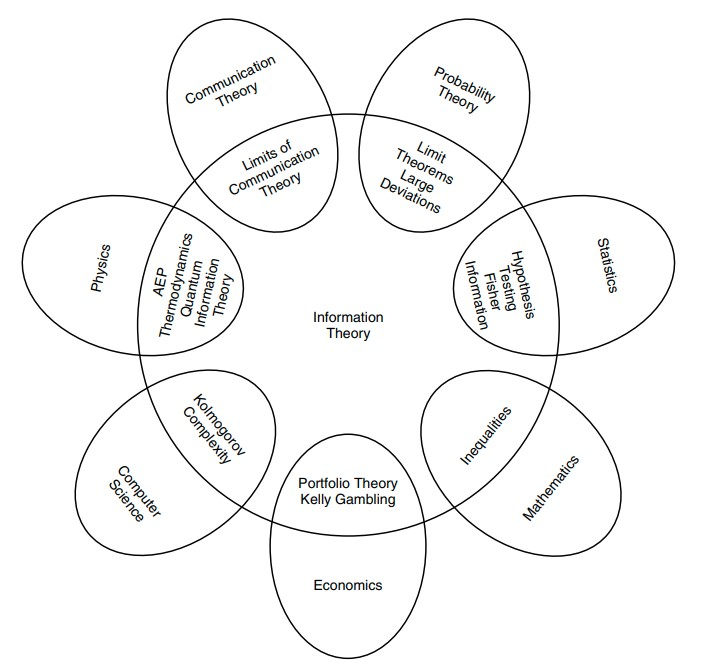
\includegraphics[width=\textwidth]{Figures/Information_theory_connections.jpg}
\caption{Connections of information theory with different science fields. Image taken from \cite{cover2006elements}}
\label{Information_theory_connections}
\end{center}
\end{figure}

\subsection{Algorithms}

Before reviewing the algorithms used in this work for the frequent item generation, we would introduce the itemset lattice: in each n-level (line) the possible combination between n elements is given (starting from 0, the void ensemble). Furthermore, each cell is connected with the cell that contains a subset of itself. The advantage of such representation will become evident during the A-priori description. There are three way by which the computational costs can be reduced: the first possibility is to reduce the number of candidates (this is the underlying idea of A-priori principle); the second option is to reduce the number of comparisons by exploiting an intelligent data structure (this is the idea of the FP growth algorithm); finally, one can reduce the number of transactions. In this work, we will consider the algorithms that use the first two approaches; thus, we would limit our theoretical analysis to these two only.


\begin{figure}
\begin{center}
\includegraphics[width=\textwidth]{Figures/itemset_lattice.jpg}
\caption{An example of itemset lattice for $I=\left\lbrace a,b,c,d,e\right\rbrace$. Image taken from \cite{tan2019introduction}}
\label{itemset_lattice}
\end{center}
\end{figure}

\paragraph{A priori}

The A-priori algorithm is based on the following principle, as stated by Tan et. al \cite{tan2019introduction}:

\begin{quote}
\textbf{A-priori principle}: If an itemset is frequent, then all of its subsets must also be frequent
\end{quote}

The support benefits of the Anti-monotone property \cite{tan2019introduction}:

\begin{quote}
\textbf{Anti-monotone property}: A measure f possesses the antimonotonone property if for every itemset X tha is a proper subset of itemset Y, i.e $X \subset Y $ we have $f(Y) \leq f(X) $
\end{quote}

Therefore, we can prune the candidates by fixing a support threshold and removing those whose subsets are not frequent enough. The crucial point, as shown in Fig. \ref{A-priori-ex} is that the algorithm starts from the smallest subset, and then, if an infrequent item is found, all the larger subset that include it are removed from the candidates. In this way the overall number of candidates is vastly reduced, thus lowering the computational cost required for the association analysis.

\begin{figure}
\begin{center}
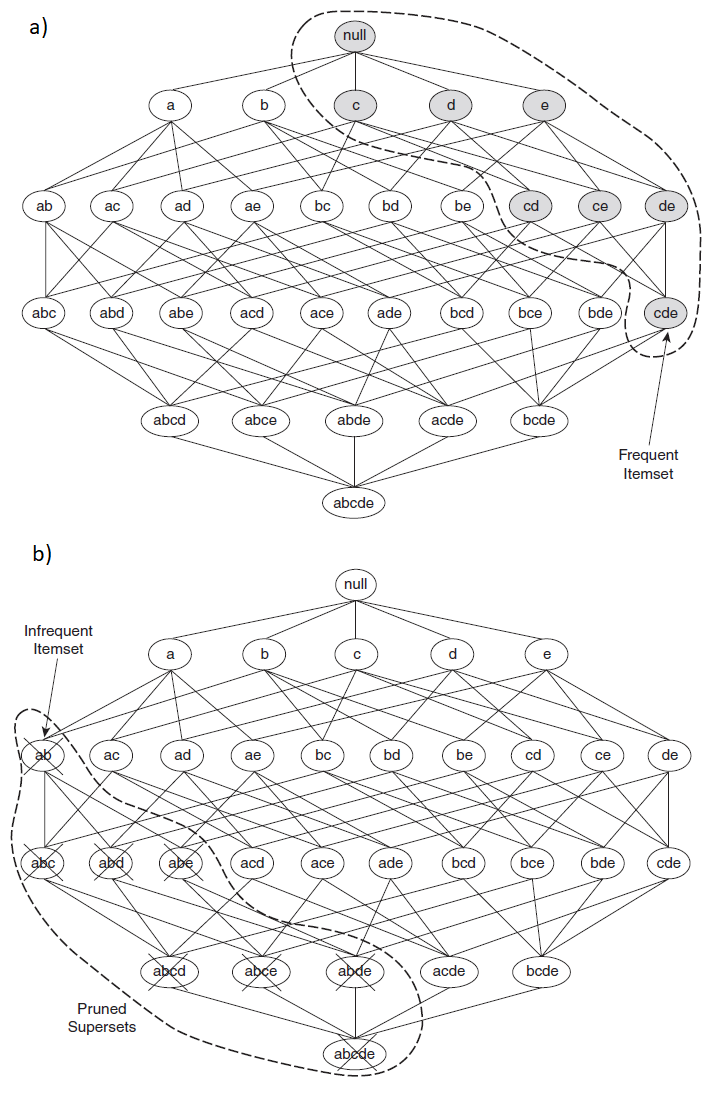
\includegraphics[width=\textwidth]{Figures/A-priori-ex.png}
\caption{The mechanism of A-priori algorithm: in the upper panel the fact that the $\left\lbrace cde \right\rbrace$ is frequent implies that the subset by which it is composed are also frequent. On this basis, one can implement an algorithm that prunes the larger itemsets by investing its subset: if a subset is infrequent, all the set that include it are also infrequent (lower panel). This approach considerably reduce the candidates and thus the computational cost of the association analysis. Images taken from \cite{tan2019introduction} }
\label{A-priori-ex}
\end{center}
\end{figure}



\paragraph{FP growth}

The Frequent Pattern (FP) algorithm represents an alternative approach to the A-priori: here, the key concept for reducing computational cost is played by how the data are stored, instead of the candidates' pruning. For this purpose, the dataset is stored into the FP-tree: this is a diagram, whose construction is explained in Fig. \ref{FP_tree} ,  in which each node represents a label of an item accompanied by a counter that reports the number of transactions mapped on the given path. The key point is that different transactions may have elements in common: thus, since some nodes in the diagram may overlap, the overall number of nodes is reduced (more precisely, we have an overlap between two paths if they have a common prefix). As we will see, the computation cost for the association analysis, given a FP-tree, depends on the number of distinct nodes: if this number is reduced, the computational effort is reduced.  Now that we described the core concept for the data compression, we move on to how the frequent itemsets are generated. This procedure is performed through a bottom-up approach in which the algorithm firstly evaluates the support for a single suffix, then evaluates the support of two element suffix, then for three element suffix, and so on. The evaluation of the support can be quickly obtained by evaluating the paths that contain a chosen node (this is why also the dashed lines were included in the diagram reported in Fig. \ref{FP_tree}). As illustrated in Fig \ref{FP_gen_1}, once a particular suffix is fixed, the algorithm generates the conditional trees that are nothing more than the part of the FP tree that verifies a particular condition i.e., to end with a particular suffix. The key point that represents one of the significant advantages of the FP algorithm is that once a particular suffix is chosen, the conditional tree that is generated provides a new subset of problems (see Fig. \ref{FP_gen_1}). In this way, the complex problem of the association analysis is attacked with a divide and conquer strategy. At this point is clear how the run-time of the FP algorithm is strictly dependent on the number of distinct nodes: if the overlap is low, the performance of this approach degrades. On the contrary, if the compression of the transaction dataset into the FP-tree is high, this method can outperform the A-priori algorithm by a different order of magnitude \cite{tan2019introduction}



\begin{figure}
\begin{center}
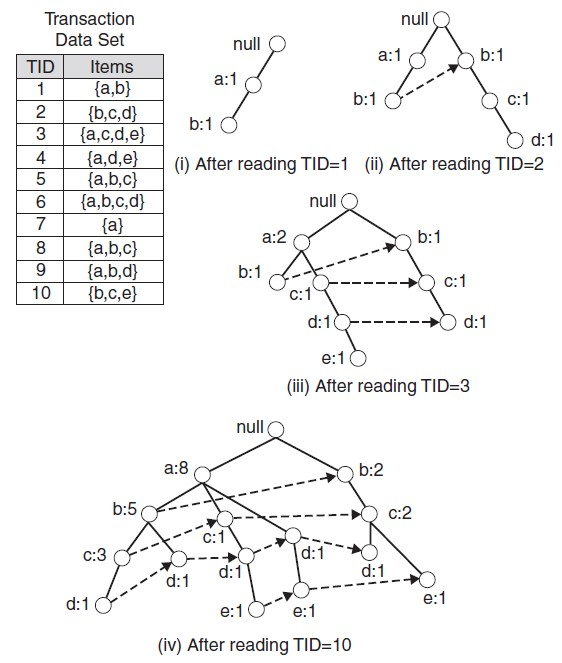
\includegraphics[width=\textwidth]{Figures/FP_tree.jpg}
\caption{The implementation of an FP-tree given a transaction. Note the dashed lines which provide the paths that connect identical elements in the diagram, but are not in the same path due to the fact that there is no common prefix.  Image taken from \cite{tan2019introduction} }
\label{FP_tree}
\end{center}
\end{figure}

\begin{figure}
\begin{center}
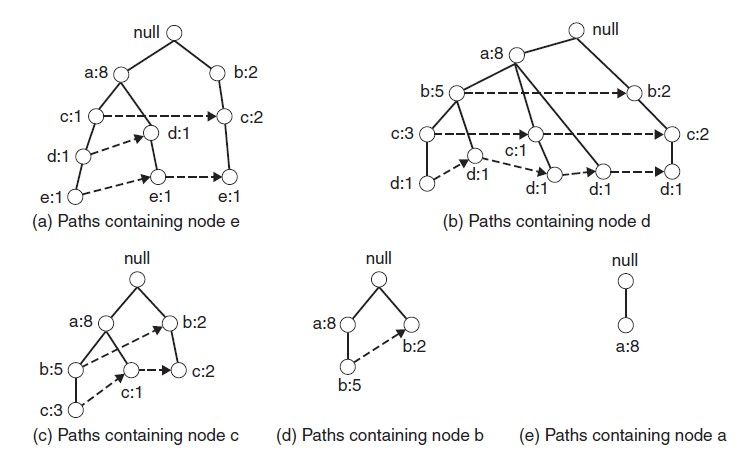
\includegraphics[width=\textwidth]{Figures/FP_gen_1.jpg}
\caption{The problem of basket analysis is decomposed into different sub-problem for each suffix. Image taken from \cite{tan2019introduction} }
\label{FP_gen_1}
\end{center}
\end{figure}

\begin{figure}
\begin{center}
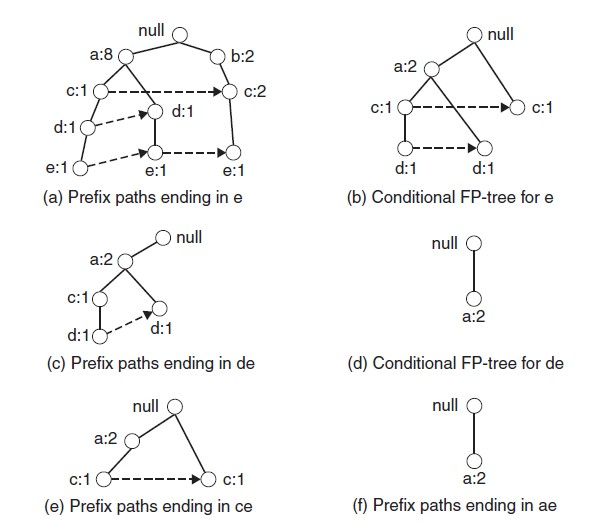
\includegraphics[width=\textwidth]{Figures/FP_gen_2.jpg}
\caption{The conditional FP-trees generated as a condition is imposed. Image taken from \cite{tan2019introduction} }
\label{FP_gen_2}
\end{center}
\end{figure}





\subsection{PCY variant}
The A-priori algorithm is characterized by a waste of memory in the first pass of the process: in fact, a considerable portion of RAM is not used, namely the amount of RAM used in the second pass to count the pairs.  The PCY variant of the A-priori algorithm uses the remaining part of the memory in the first pass to reduce the candidates. In fact, it constructs a hash table on the first pass, using all main-memory space that is not needed to count the items. Pairs of items are hashed to be mapped into buckets; the buckets are used as counters of the number of times a pair hashed to that bucket. On the second pass, we only have to count pairs of frequent items that hashed to a frequent bucket (one whose count is at least the support threshold) on the first pass.
}


\begin{figure}[ht]
  \fbox{\begin{minipage}[b]{0.5\linewidth}
    \centering
    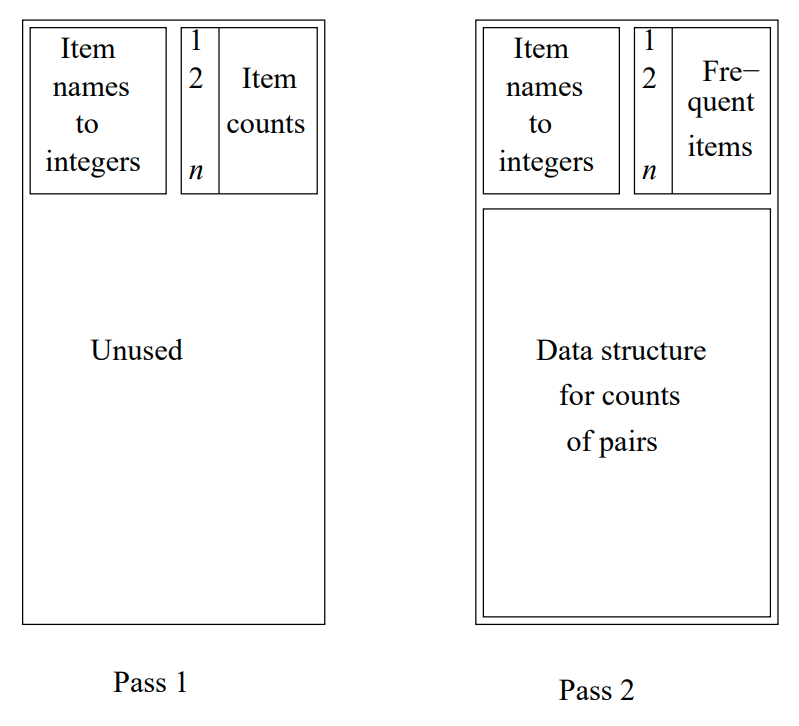
\includegraphics[width=.9\linewidth]{Figures/Apriori_memory.png}
    \subcaption{A-priori}
    \vspace{4ex}
  \end{minipage} }
  \fbox{\begin{minipage}[b]{0.5\linewidth}
    \centering
    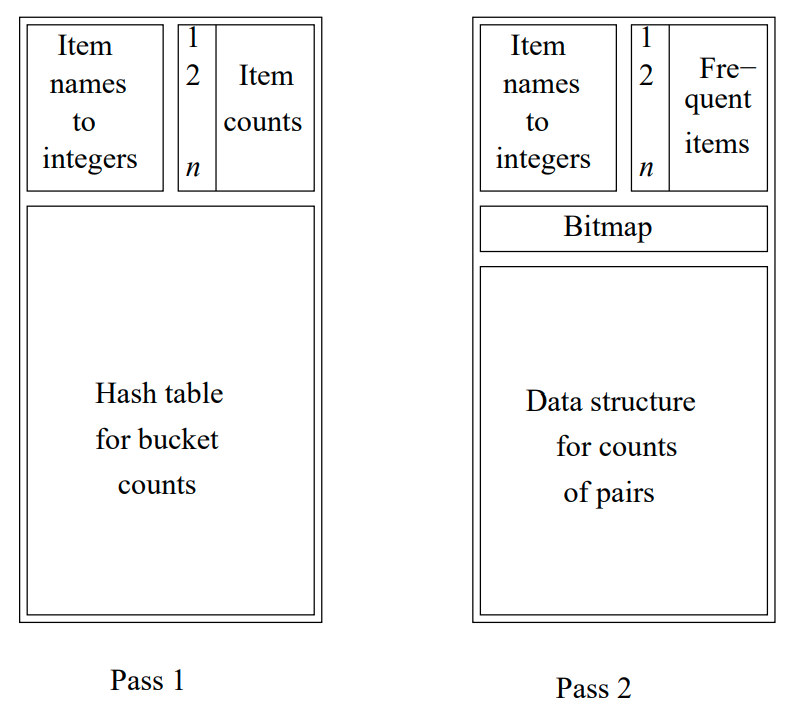
\includegraphics[width=.9\linewidth]{Figures/PCY_memory.png}
    \subcaption{PCY}
    \vspace{4ex}
  \end{minipage}}%%
\caption{Use of memory for A-priori algorithm and for PCY variant. Image taken from \cite{leskovec2020mining}}
\label{Support distribution_ALL}
\end{figure}



\chapter{Dataset generation}

\section{Tweet retrieval}

Twitter and other social media platforms represent an important and updated source of information with regard to the development of our society, since social media platforms generate a vast amount of data daily on a variety of topics. Therefore, it is important to be able to retrieve tweets in order to be able to analyze them. In order to reach this goal, Twitter offers companies, developers, and users programmatic access to Twitter data through API (Application Programming Interfaces). Using the Twitter APIs, developers can access public Tweets by searching for specific keywords \cite{twitter}. To retrieve all tweets with a specific hashtag, it is possible to use the search/tweets GET endpoint. By default, the results return tweets sent in the previous seven days. Tweets are delivered in reverse-chronological order, starting with the most recent.  Therefore, the sample extracted can not be considered,  in principle,  a random one.  However, under the condition that there is no particular event from the first to the last tweet extracted that alters the association,\footnote{We verified that this condition was true from different on-line press agencies } we can consider the sample as randomly extracted.  Furthermore, it is also possible to select the language of the tweets. The resulting csv file is available in the following format: hashtag|timestamp|tweet\_text|user\_name|language . For the purpose of our project, only  the tweet\_text is necessary, since we will consider each tweet as a basket and the words contained in them as the items.

\section{Choice of the dataset}

We chose to work on five datasets composed of 10000 tweets that contain respectively the following hashtags: \textit{freedom, Afghanistan, rare earth, Covid-19 and Pfizer}\footnote{Retrieved starting from 26/08/2021 to 28/08/2021}.  The ratio behind the choice of the hashtag has been to have tweets with several levels of specificity and technicality, and concerning different topical questions, in particular the Afghanistan crisis and the pandemic situation. The hashtag \textit{freedom} is a generic hashtag that can be linked both with the rise to power of the Taliban regime and with the possibility to make vaccination compulsory.  \textit{delta}, \textit{Pfizer} and \textit{vaccines} are related to the pandemic,  but they show a different level of technicality, since vaccines is a common word while the others two refer to a more technical field, even if they have become very popular in the public debate.  \textit{Afghanistan} and \textit{rare earth } refer to the Afghanistan situation: in this case, the latter shows a high level of specificity since it is about an issue that is not widely known, namely the interest of some countries to exploit Afghanistan’s rare earth metals, some crucial elements in modern technology.


\chapter{Results and discussion}

For each term, we conducted a preliminary analysis on its cleaned document-term matrix: as it is possible to point out from Fig. \ref{Matrix_ALL}, a sparse matrix was obtained, as expected,  for each hashtag.  We then applied the FP-growth algorithm,  as implemented in Spark suite of codes \cite{zaharia2016apache} ,  and the A-priori algorithm,  as implemented in MLxtend suite of codes \cite{raschka2018mlxtend}. With the first one, we retrieved the frequency for each itemset,  the association rule for each basket, and the predictions of the items that are most likely to appear given a basket.  A support threshold equal to 0.03 was chosen. A preview of the results is given in the Tab. \ref{POP_RareEarth}, \ref{POP_Afghanistan}, \ref{POP_Delta}, \ref{POP_Pfizer},\ref{POP_Vaccines} and \ref{POP_Freedom}  for the 5 most popular items, while the associations (the five with the higher lifts) are given in \ref{ASS_RareEarth}, \ref{ASS_Afghanistan}, \ref{ASS_Delta}, \ref{ASS_Pfizer} and \ref{ASS_Vaccine} (note that the table for hashtag freedom is not present since there is no association with a support equal to 0.03). It is worth noting that in the pre-processing phase the hashtag was removed, thus the singleton represents, in this perspective, a binary combination between the word of the hashtag and the singleton itself. For this reason, in our analysis we will consider as multiple association a combination of two or more words, since the hashtag is implicitly included in the association. The full results (in the form of an Excel table) obtained for each hashtag are provided here \cite{Folder},  and a good visual representation of them is provided in Fig. \ref{Support distribution_ALL} and Fig. \ref{WordCloud_ALL}.  Let us start from the Rare earth hashtag, that present a large number of high frequency peaks given by the words \textit{minerals, china, Afghanistan, metals} and \textit{taliban} (see Tab. \ref{POP_RareEarth}): the presence of the words China, Afghanistan and talibans is associated with this hashtag due to the interest of some countries, such as China, to exploit Afghanistan’s rare earth metals. Furthermore, also the multiple association table Tab. \ref{POP_RareEarth}, in which we see a high lift value for the association \textit{lithium} and \textit{copper}, provide interesting informations: in fact, this association is due to the fact that these two metals are largely present in Afghanistan together with rare earth \footnote{The reader must be aware that lithium and copper are not rare-earth. A full discussion about the chemistry and the industrial uses of these materials can be found into a general chemistry textbook such as \cite{petrucci2010general}}. In the case of the Afghanistan hashtag, we have a support distribution with a very sharp peak connected to \textit{Taliban} and \textit{Kabul}: while the first one is connected because it is the Afghanistan capital (see Tab. \ref{POP_Afghanistan}), the second one is an effect of Taliban conquer of Afghanistan happened at the end of August 2021, after US troops withdraw. The importance of the US in the political scenario of the Afghanistan is also captured by the words \textit{us}, \textit{biden}, while the association between Afghanistan and \textit{kabulairport} is given both by the importance of this place for the evacuation of the US troops and by the terroristic attack that took place during the evacuation. These words and their associations provide the first peak and the second broader one. Looking to the multiple associations table (Tab. \ref{ASS_Afghanistan}), we can see that the association with larger lift is given by \textit{nowazd} and \textit{usarmy}; this connection is due to the Nowzad Dogs charity, whose supporters provided financial support for the evacuation of the association staff and their animals \cite{Nowzad}. The following association are basically connected with the capture of Kabul by Taliban and the civilian evacuation. Concerning the hashtag delta, we can see that we have an overall sharp peak made firstly by the words \textit{covid19},\textit{covid}, \textit{variant}, \textit{amp} and \textit{vaccine} (see Tab. \ref{POP_Delta}). These findings clearly signal the extensive use of word delta within the pandemic framework, while other fields in which this word appears, such as, for instance, the delta airlines, does not contribute to the spread of this hashtag in the social media. An inspection of the multiple associations between the word delta and other words, reported in Tab \ref{ASS_Delta}, highlights the words \textit{vaccine}, \textit{covid19} and \textit{variant}: however, in contrast to the previous case (hashtag Afghanistan), we can note that the maximum lift is very close to 1, thus the interest of these associations is poor. Moving to the hashtag pfizer, we see that we have a very sharp peak connected with the term \textit{vaccine}, followed by \textit{covid19}, \textit{fda} (food and drug administration) and by the association \textit{covid19,vaccine}. In this case, as we can note looking to Tab \ref{ASS_Pfizer}, we have an interesting lift value for \textit{full,vaccine}: this is the effect of the public debate about the vaccination campaign, also connected with the discussion on the possibility of a third dose, as one can see from the lift value of the association \textit{full, approval}. Concerning the hashtag vaccines, we point out the presence of large peak at the origin connected with the word \textit{covid19}, followed by \textit{covid} and \textit{amp}. With regards to the multiple association, we can see that these has a lift value close to 1. Finally, the distribution connected with freedom is almost horizontal, highlighting that this hashtag is associated with several fields, and therefore a low information content can be retrieved with it. The lack of interesting associations is also captured by the fact that no multiple association with a support equal or larger with respect to 0.03 is present, thus in this case not table is provided. In order to quantify this contrast, we propose to evaluate the area under the support curve (remembering that the curves here reported refer only to the itemsets whose support is larger than the chosen threshold): the idea is that if this area is low, the specificity of the hashtag searched is very low; on the contrary, if the area is high we have a higher level of specificity (i.e. only a few words are usually combined with a hashtag with the high area). From an information theory point of view, the first case corresponds to a large entropy (every state is equally probable), the second one to low entropy (few probable states). The results of this evaluation for the hashtags here considered are provided in Tab. \ref{TAB_area}: the RareEarth is associated with the higher value, followed by Afghanistan and Pfizer; on the other side, freedom has low specificity since it can be associated with a cumbersome amount of words. In the author's view, the area can be considered as an assessment of the information content obtained by mining tweets with this word: if a hashtag w with a high area (above the support threshold) is used, it is associated almost with specific terms. Thus the tweets retrieved used with this hashtag were will more likely to provide useful information. On the other side, a hashtag connected with a low area will provide many spurious tweets, and thus, in the end, no useful information will be retrieved.

\begin{figure}[ht]
  \begin{minipage}[b]{0.5\linewidth}
    \centering
    
\includegraphics[width=.9\linewidth]{Figures/Matrix_rareearth.jpg}
    \subcaption{rareearth}
    \vspace{4ex}
  \end{minipage}
  \begin{minipage}[b]{0.5\linewidth}
    \centering
    
\includegraphics[width=.9\linewidth]{Figures/Matrix_afghanistan.jpg}
    \subcaption{Afghanistan}
    \vspace{4ex}
  \end{minipage}
  \begin{minipage}[b]{0.5\linewidth}
    \centering
    
\includegraphics[width=.9\linewidth]{Figures/Matrix_delta.jpg}
    \subcaption{Delta}
    \vspace{4ex}
  \end{minipage}
    \begin{minipage}[b]{0.5\linewidth}
    \centering
    
\includegraphics[width=.9\linewidth]{Figures/Matrix_pfizer.jpg}
    \subcaption{Pfizer}
    \vspace{4ex}
  \end{minipage}
  \begin{minipage}[b]{0.5\linewidth}
    \centering
    
\includegraphics[width=.9\linewidth]{Figures/Matrix_vaccine.jpg}
    \subcaption{Vaccine}
    \vspace{4ex}
  \end{minipage}
  \begin{minipage}[b]{0.5\linewidth}
    \centering
    
\includegraphics[width=.9\linewidth]{Figures/Matrix_freedom.jpg}
    \subcaption{freedom}
    \vspace{4ex}
  \end{minipage}

\caption{Document-term matrix for the different hashtags. The high quality ones are available at \cite{Folder}}
\label{Matrix_ALL}
\end{figure}


\begin{figure}[ht]
   \begin{minipage}[b]{0.5\linewidth}
   \centering
    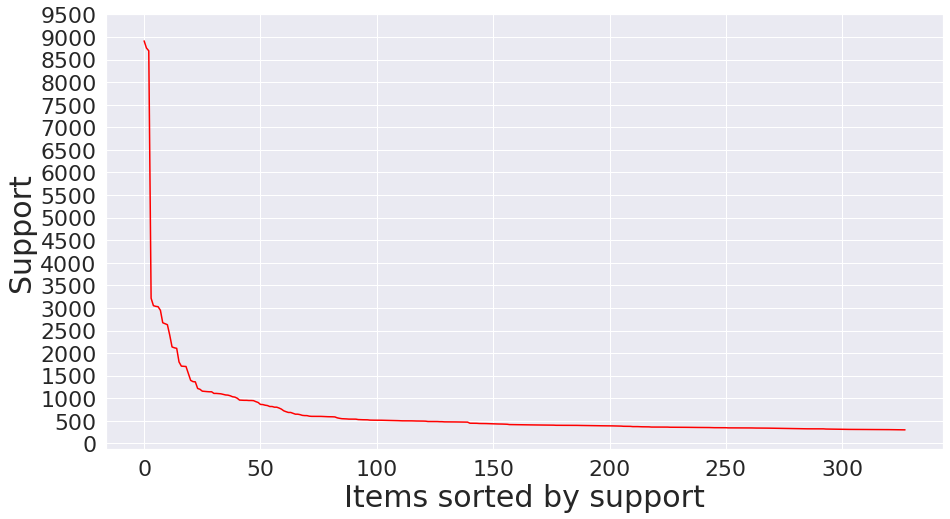
\includegraphics[width=.9\linewidth]{Figures/Support_distrubution_Rareearth.png}
    \subcaption{Rareearth}
    \vspace{4ex}
  \end{minipage}
  \begin{minipage}[b]{0.5\linewidth}
    \centering
    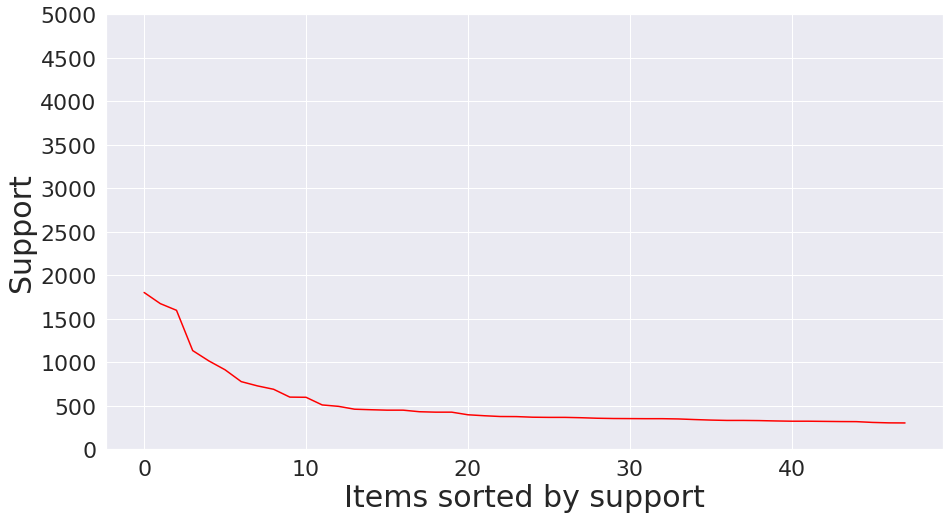
\includegraphics[width=.9\linewidth]{Figures/Support_distrubution_Afghanistan.png}
    \subcaption{Afghanistan}
    \vspace{4ex}
  \end{minipage}
  \begin{minipage}[b]{0.5\linewidth}
    \centering
    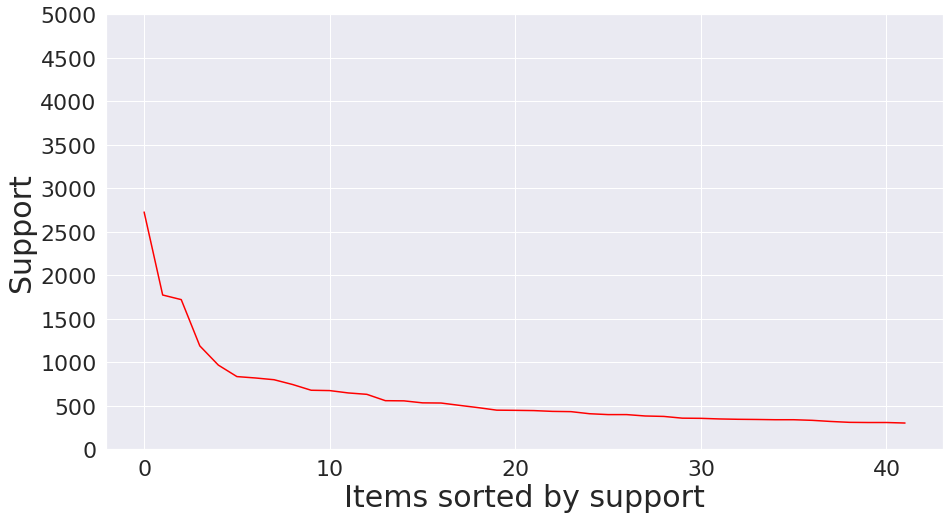
\includegraphics[width=.9\linewidth]{Figures/Support_distrubution_delta.png}
    \subcaption{Delta}
    \vspace{4ex}
  \end{minipage}
    \begin{minipage}[b]{0.5\linewidth}
    \centering
    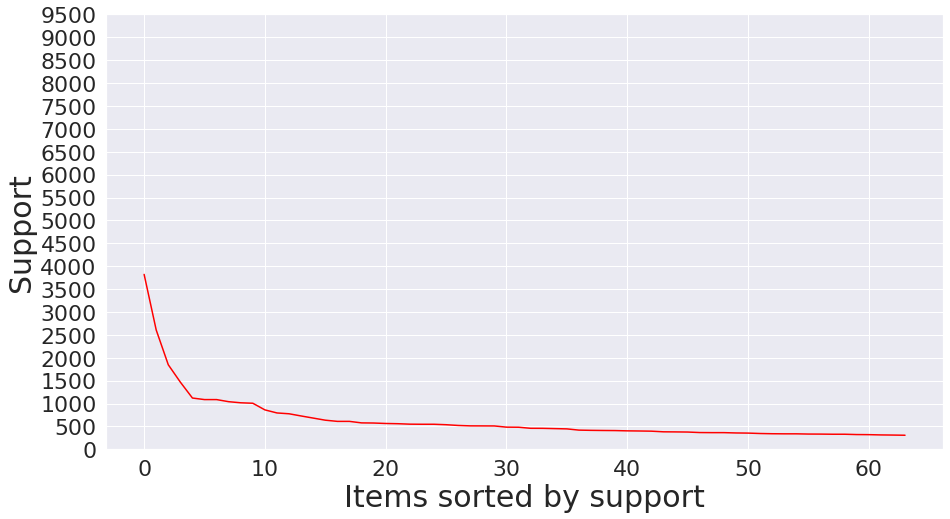
\includegraphics[width=.9\linewidth]{Figures/Support_distrubution_pfizer.png}
    \subcaption{Pfizer}
    \vspace{4ex}
  \end{minipage}
  \begin{minipage}[b]{0.5\linewidth}
    \centering
    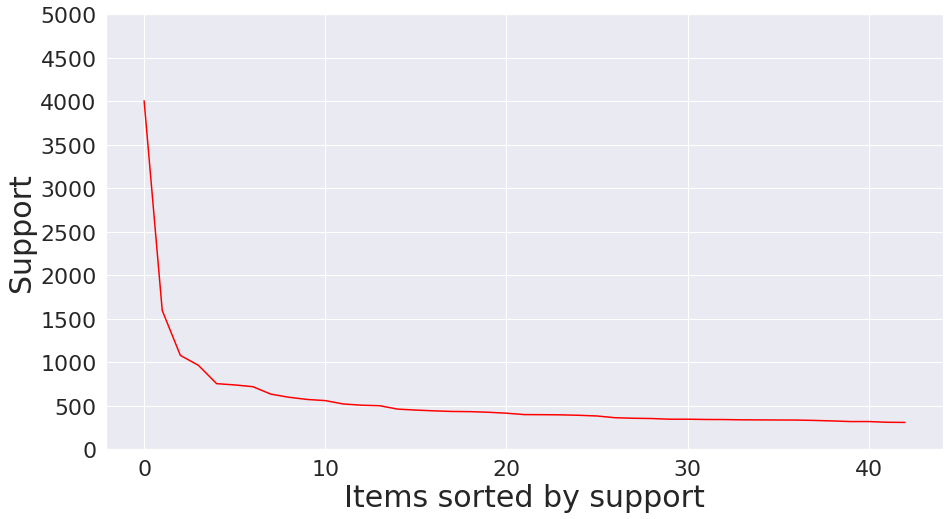
\includegraphics[width=.9\linewidth]{Figures/Support_distrubution_Vaccine.png}
    \subcaption{Vaccines}
    \vspace{4ex}
  \end{minipage}%%
     \begin{minipage}[b]{0.5\linewidth}
    \centering
    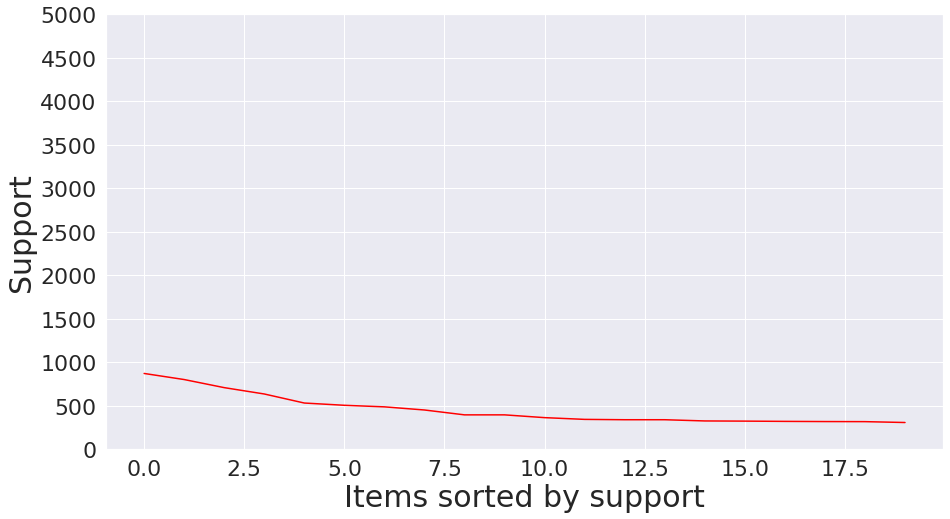
\includegraphics[width=.9\linewidth]{Figures/Support_distrubution_Freedom.png}
    \subcaption{Freedom}
    \vspace{4ex}
  \end{minipage}

\caption{Support distribution for the different hashtags}
\label{Support distribution_ALL}
\end{figure}


\begin{figure}[ht]
   \begin{minipage}[b]{0.5\linewidth}
    \centering
    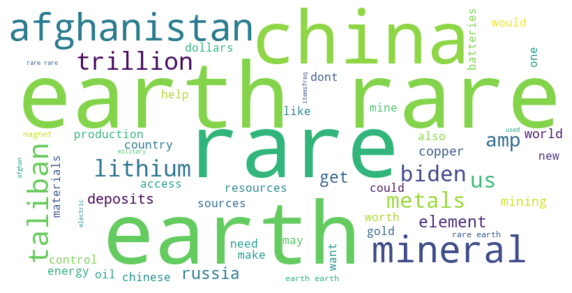
\includegraphics[width=.9\linewidth]{Figures/WordCloud_Rareearth.png}
    \subcaption{Rareearth}
    \vspace{4ex}
  \end{minipage}
  \begin{minipage}[b]{0.5\linewidth}
    \centering
    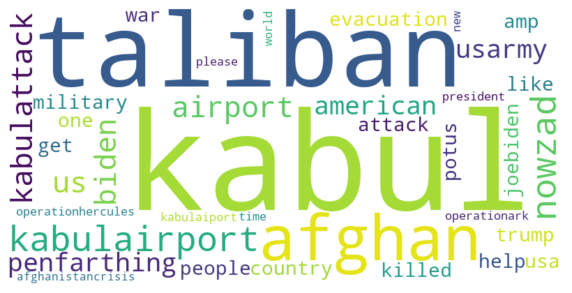
\includegraphics[width=.9\linewidth]{Figures/WordCloud_Afghanistan.png}
    \subcaption{Afghanistan}
    \vspace{4ex}
  \end{minipage}
  \begin{minipage}[b]{0.5\linewidth}
    \centering
    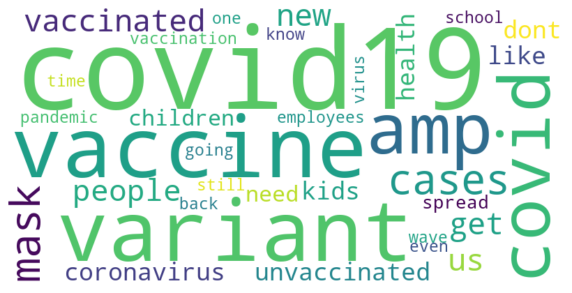
\includegraphics[width=.9\linewidth]{Figures/WordCloud_delta.png}
    \subcaption{Delta}
    \vspace{4ex}
  \end{minipage}
    \begin{minipage}[b]{0.5\linewidth}
    \centering
    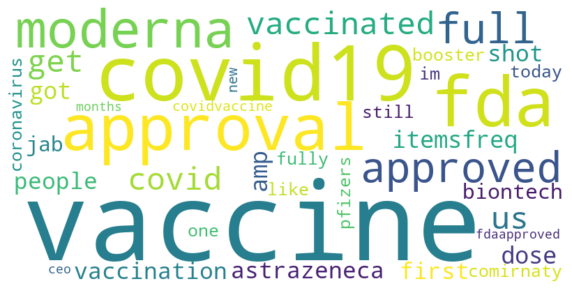
\includegraphics[width=.9\linewidth]{Figures/WordCloud_pfizer.png}
    \subcaption{Pfizer}
    \vspace{4ex}
  \end{minipage}
  \begin{minipage}[b]{0.5\linewidth}
    \centering
    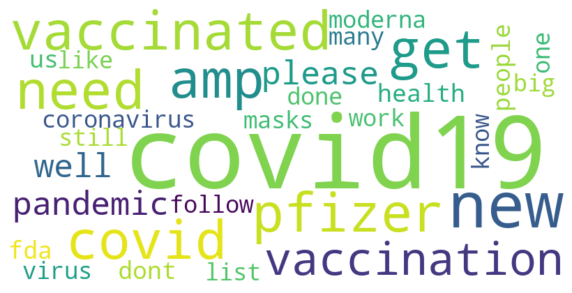
\includegraphics[width=.9\linewidth]{Figures/WordCloud_Vaccine.png}
    \subcaption{Vaccines}
    \vspace{4ex}
  \end{minipage}
     \begin{minipage}[b]{0.5\linewidth}
    \centering
    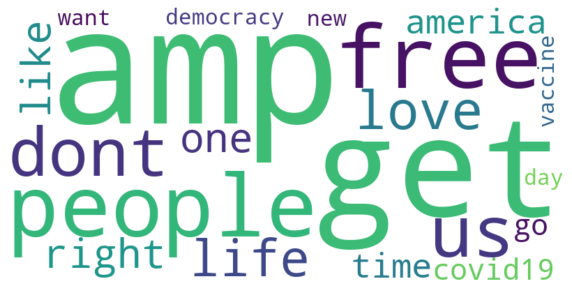
\includegraphics[width=.9\linewidth]{Figures/WordCloud_Freedom.png}
    \subcaption{Freedom}
    \vspace{4ex}
  \end{minipage}
\caption{WordCloud for the different hashtags}
\label{WordCloud_ALL}
\end{figure}


\begin{table}[]
\caption{Most popular items for hashtag \textit{RareEarth}}
\begin{center}
\begin{tabular}{l|l}
            & \textbf{Support} \\ \hline
Minerals    & 3215    \\ \hline
China       & 2948    \\ \hline
Afghanistan & 2400    \\ \hline
Metals      & 1804    \\ \hline
Taliban     & 1551    \\ \hline
Us          & 1217
\label{POP_RareEarth}
\end{tabular}
\end{center}
\end{table}

\begin{table}[]
\caption{Most popular items for hashtag \textit{Afghanistan}}
\begin{center}
\begin{tabular}{l|l}
        & \textbf{Support} \\ \hline
Taliban & 1803 \\ \hline
Kabul   & 1675 \\ \hline
Us      & 1598 \\ \hline
Biden   & 1135 \\ \hline
Amp     & 1016 \\ \hline
Afghan  & 914
\label{POP_Afghanistan}
\end{tabular}
\end{center}
\end{table}


\begin{table}[]
\caption{Most popular items for hashtag \textit{Delta}}
\begin{center}
\begin{tabular}{l|l}
        & \textbf{Support} \\ \hline
Covid19 & 2728    \\ \hline
Covid   & 1774    \\ \hline
Variant & 1721    \\ \hline
Amp     & 1189    \\ \hline
Vaccine & 968     \\ \hline
Cases   & 836
\label{POP_Delta}
\end{tabular}
\end{center}
\end{table}
\begin{table}[]
\caption{Most popular items for hashtag \textit{Pfizer}}
\begin{center}
\begin{tabular}{l|l}
         & \textbf{Support} \\ \hline
Vaccine  & 3821    \\ \hline
Covid19  & 2607    \\ \hline
Fda      & 1847    \\ \hline
Covid19  & 1467    \\ \hline
Approval & 1120    \\ \hline
Moderna  & 1086
\label{POP_Pfizer}
\end{tabular}
\end{center}
\end{table}

\begin{table}[]
\caption{Most popular items for hashtag \textit{Vaccines}}
\begin{center}
\begin{tabular}{l|l}
           & \textbf{Support} \\ \hline
Covid19    & 4007    \\ \hline
Covid      & 1596    \\ \hline
Amp        & 1080    \\ \hline
Get        & 965     \\ \hline
People     & 755     \\ \hline
Vaccinated & 740
\label{POP_Vaccines}
\end{tabular}
\end{center}
\end{table}
\begin{table}[]
\caption{Most popular items for hashtag \textit{Freedom}}
\begin{center}
\begin{tabular}{l|l}
       &\textbf{ Support} \\ \hline
Amp    & 872     \\ \hline
Get    & 802     \\ \hline
People & 709     \\ \hline
Free   & 636     \\ \hline
Us     & 532     \\ \hline
Dont   & 506
\label{POP_Freedom}
\end{tabular}
\end{center}
\end{table}



\begin{table}[]
\caption{Association rule for the hashtag \textit{RareEarth}}
\begin{tabular}{l|l|l|l|l}
\textbf{Antecedent} & \textbf{Consequent}  & \textbf{Lift} & \textbf{Confidence} & \textbf{Support }\\ \hline
lithium     & copper      & 6.07 & 0.27       & 0.03    \\ \hline
deposits    & lithium     & 4.56 & 0.53       & 0.03    \\ \hline
russia      & china       & 2.99 & 0.88       & 0.04    \\ \hline
china       & afghanistan & 2.62 & 0.13       & 0.04    \\ \hline
afghanistan & biden       & 2.44 & 0.14       & 0.03
\label{ASS_RareEarth}
\end{tabular}
\end{table}


\begin{table}[]
\caption{Association rule for the hashtag \textit{Afghanistan}}
\begin{tabular}{l|l|l|l|l}
\textbf{Antecedent} & \textbf{Consequent}  & \textbf{Lift} & \textbf{Confidence} & \textbf{Support}\\ \hline
nowzad       & usarmy       & 21.16 & 0.68       & 0.03    \\ \hline
nowzad       & penfarthing  & 16.80 & 0.72       & 0.03    \\ \hline
kabulattack  & kabulairport & 9.01  & 0.70       & 0.03    \\ \hline
airport      & kabul        & 4.60  & 0.77       & 0.05    \\ \hline
kabulairport & kabul        & 3.49  & 0.27       & 0.05
\label{ASS_Afghanistan}
\end{tabular}
\end{table}

\begin{table}[]
\caption{Association rule for the hashtag \textit{Delta}}
\begin{tabular}{l|l|l|l|l}
\textbf{Antecedent} & \textbf{Consequent}  & \textbf{Lift} & \textbf{Confidence} & \textbf{Support }\\ \hline
vaccine    & covid19    & 1.65 & 0.45       & 0.04    \\ \hline
covid19    & cases      & 1.40 & 0.12       & 0.03    \\ \hline
covid19    & variant    & 1.38 & 0.24       & 0.06    \\ \hline
covid19    & covid      & 1.15 & 0.20       & 0.06    \\ \hline
amp        & covid19    & 0.95 & 0.26       & 0.03
\label{ASS_Delta}
\end{tabular}
\end{table}


\begin{table}[]
\caption{Association rule for the hashtag \textit{Pfizer}}
\begin{tabular}{l|l|l|l|l}
\textbf{Antecedent} & \textbf{Consequent}  & \textbf{Lift} & \textbf{Confidence} & \textbf{Support}\\ \hline
full,vaccine     & approval   & 8.19 & 0.92       & 0.04    \\ \hline
full             & approval   & 7.08 & 0.79       & 0.05    \\ \hline
approved,vaccine & fda        & 3.97 & 0.73       & 0.04    \\ \hline
approval,covid19 & vaccine    & 2.18 & 0.83       & 0.03    \\ \hline
full, approval   & vaccine    & 2.04 & 0.78       & 0.04

\label{ASS_Pfizer}
\end{tabular}
\end{table}

\begin{table}[]
\caption{Association rule for the hashtag \textit{Vaccine}}
\begin{tabular}{l|l|l|l|l}
\textbf{Antecedent} & \textbf{Consequent}  & \textbf{Lift} & \textbf{Confidence} & \textbf{Support }\\ \hline
covid19    & please     & 1.96 & 0.08       & 0.03    \\ \hline
news       & covid19    & 1.91 & 0.76       & 0.03    \\ \hline
covid19    & well       & 1.84 & 0.08       & 0.03    \\ \hline
covid19    & pandemic   & 1.64 & 0.09       & 0.03    \\ \hline
covid19    & need       & 1.56 & 0.10       & 0.04
\label{ASS_Vaccine}
\end{tabular}
\end{table}





\begin{table}[]
\begin{center}
\caption{Area under the support distribution curve normalized by the lowest value (Freedom). Note that the items with support lower with respect to the threshold 0.03 were discarded}
\begin{tabular}{l|l}
            & Area  \\ \hline
RareEarth   & 6.14 \\ \hline
Afghanistan & 4.60  \\ \hline
Pfizer      & 2.86  \\ \hline
Vaccines    & 2.85  \\ \hline
Delta       & 2.63  \\ \hline
Freedom     & 1.00     \\
\label{TAB_area}
\end{tabular}
\end{center}
\end{table}








\chapter{Conclusion}
From the basket analysis that we conducted on the datasets that we generated from a set of hashtags through the Twitter APIs, we saw that a given hashtag can involve words that can span from a single very specific area of interest to many fields. The first case is what happens with the  \textit{RareEarth} hashtag, the second one with the \textit{Freedom} one. The shape of the support distribution captures such behaviour: a horizontal one (high entropy) highlights a word that is used in an extensive set of context, while a distribution with a high peak at the origin (low entropy) highlight a word that is used into a very reduced context. Since the quality of information is linked to the specificity of words used with it, we propose to use the overall area under the support distribution (once the area below the support is removed) to assets numerically the information quality connected with a particular hashtag: in this framework, the behaviour of \textit{RareEarth} hashtag is emblematic since it is more specific and technical with respect to \textit{freedom} that can be used almost in every context.



\bibliographystyle{unsrt}

\bibliography{sample.bib} % The file containing the bibliography

\newpage




%----------------------------------------------------------------------------------------

\end{document}
